% DevMind term-project report draft based on the faculty-provided
% Procedia Computer Science LaTeX template. Team metadata remains to be filled.
% Compile from this folder with: pdflatex DevMind_Term_Report.tex (twice).
\documentclass[3p,times,procedia]{elsarticle}
\flushbottom
\usepackage{ecrc}
\usepackage[bookmarks=false]{hyperref}
\hypersetup{colorlinks,linkcolor=blue,citecolor=blue,urlcolor=blue}
\usepackage{amssymb}
\usepackage[figuresright]{rotating}
\usepackage{graphicx}
\usepackage{booktabs}
\usepackage{array}
\biboptions{numbers,sort&compress}

\volume{00}
\firstpage{1}
\journalname{Procedia Computer Science}
\runauth{DevMind Team}
\jid{procs}

\begin{document}
\begin{frontmatter}
\dochead{International Conference on Machine Learning and Data Engineering}
\title{DevMind: An Evidence-Grounded Framework for Explainable Bug Analysis, Repository Localization and Sandboxed Software Repair}

% Names and roll numbers follow the existing project presentation; confirm
% spelling and author order with the team before submission.
\author[a]{P. Sharath Chandhra}
\author[a]{B. Shashank Manohar}
\author[a]{K. Venkat Sai Mani Avinash}
\address[a]{Department of Computer Science and Engineering, [College/University], [City], India}

\begin{abstract}
Software bug reports describe symptoms in natural language, while relevant evidence is distributed across repository files and tests. DevMind is a local repository-analysis prototype that combines deterministic issue-text processing, traceable source retrieval, optional model-generated patch candidates, and Docker-based testing of disposable copies. Its application defaults to TF--IDF cosine retrieval; a pinned CPU experiment compared it with local dense retrieval on five SWE-bench Lite development issues from five repositories. Against one unreviewed changed-file proxy per issue, mean raw-query Recall@5 was 0.80 for TF--IDF and 0.40 for dense cosine; mean P@1 was 0.40 for both. Dense document embedding and index construction took 594.737 seconds, versus 1.199 seconds for TF--IDF index construction in the same run. These descriptive results do not establish general effectiveness because annotations are weak and the sample is small. The Task Analyzer is rule-based, not a trained classifier, and DevMind has no official SWE-bench grade. We report the measured pilot and its limits rather than infer repair effectiveness from retrieval results.\end{abstract}

\begin{keyword}
text analytics \sep software bug analysis \sep TF--IDF retrieval \sep code repair \sep sandbox testing \sep evidence traceability
\end{keyword}
\end{frontmatter}
% TODO: Add the confirmed corresponding-author marker, contact note, and email
% after the team approves the author order and contact details.

\section{Introduction}
Software maintenance begins with incomplete reports: a user describes an observed failure, but the cause may lie in a function, its callers, configuration, or an existing test. Repository-level repair systems therefore need more than code generation. They must locate relevant context, preserve evidence provenance, and distinguish a proposed change from a change that has been tested.

Retrieval-augmented generation (RAG) combines a language model with retrieved external evidence, while repository issue benchmarks such as SWE-bench evaluate whether a proposed change resolves real GitHub issues under project tests \cite{Lewis2020,Jimenez2024}. Systems including SWE-agent and AutoCodeRover show how tool interfaces, repository navigation, and test execution can support software-engineering agents \cite{Yang2024,Zhang2024}. These works motivate repository-aware assistance, but their results do not transfer automatically to a smaller student prototype or a different model and test environment.

DevMind explores a practical workflow for a developer who provides a bug report and a local repository or public GitHub URL. The system analyzes issue text, statically indexes supported source files, retrieves ranked code evidence, and can request an optional model-generated patch. Testing occurs only in a disposable Docker copy. The study focuses on the implemented pipeline and the evidence available in recorded runs. It does not claim that the text analyzer is learned, that the five-case dense comparison establishes general retrieval effectiveness, or that DevMind has a SWE-bench resolution score.

\section{Problem Definition and Objectives}
Given a natural-language bug report $q$ and a repository snapshot $R$, DevMind aims to produce (1) structured issue features, (2) a ranked set of source evidence with file and line provenance, and (3) optionally, a reviewable patch candidate with an isolated test outcome. A successful run must report blockers honestly: a generated patch is not a verified fix, and passing selected tests is not proof that the issue is resolved in all relevant conditions.

The implemented objectives are to normalize and summarize issue text; retrieve code locations without importing target code; make optional model calls replaceable and bounded; validate candidate diffs; test candidates in a network-restricted disposable environment; and record evidence and limitations in a machine-readable report. The project also includes a comparison runner and a SWE-bench Lite prediction adapter, but their existence does not mean their intended experiments have been completed.

\section{Related Work}
RAG combines language-model generation with retrieved external evidence \cite{Lewis2020}. In repository software engineering, SWE-bench established issue-linked patch evaluation against repository tests \cite{Jimenez2024}; SWE-agent studies tool interfaces for navigating and modifying repositories \cite{Yang2024}; AutoCodeRover uses structured repository search and test-guided localization \cite{Zhang2024}; and Agentless evaluates a structured localization, repair, and validation pipeline \cite{Agentless2025}. These systems establish repository-level repair and evaluation as active areas, but their model, benchmark, and tool results do not transfer to DevMind.

RepairAgent evaluates a finite-state LLM repair workflow on Java defects, while RepoAI studies multi-agent retrieval-augmented code refactoring \cite{RepairAgent2025,RepoAI2026}. These are related but distinct tasks; DevMind is not a multi-agent system, and no results from those studies are attributed to it. Bug-report classification is also established: a large cross-project study and a systematic review describe supervised classifiers and common lexical representations such as TF--IDF \cite{Andrade2026,Long2025}. DevMind's exact-token category rules remain untrained and unevaluated on an independent labelled corpus.

Bug-report query reformulation and ranking have also been studied directly. BRaIn uses relevance feedback to reformulate localization queries \cite{BRaIn2025}, while a 2026 workshop preprint studies identifier and code-cue extraction followed by BM25 retrieval \cite{Reformulate2026}. IQLoc investigates semantics-driven query reduction for bug localization \cite{IQLoc2026}; SpIDER combines dense retrieval with structural expansion \cite{SpIDER2026}. Evidence-guided repair and the relationship between localization and repair outcomes have also received direct study, including EviACT and Loc2Repair \cite{EviACT2026,Loc2Repair2026}. Thus, DevMind does not claim novelty for query reformulation, lexical/semantic/hybrid retrieval, bounded repair, or the general hypothesis that localization can affect repair.

DevMind's current engineering contribution is a traceable implementation of four deterministic query conditions and a local evaluator that compares lexical and dense retrieval on the same indexed chunks. The five-case pilot is an initial descriptive comparison, not a validated effectiveness claim: its changed-file proxies are not independently reviewed fault locations.

\begin{table}[t]
\caption{Selected related work and its relationship to DevMind (ACR: AutoCodeRover; RRL: Reformulate, Retrieve, Localize).}
\label{tab:related-work}
\centering
\small
\begin{tabular*}{\linewidth}{@{\extracolsep{\fill}}>{\raggedright\arraybackslash}p{0.26\linewidth}>{\raggedright\arraybackslash}p{0.42\linewidth}>{\raggedright\arraybackslash}p{0.25\linewidth}@{}}
\toprule
Work & Established task or method & Relationship to DevMind \\
\midrule
SWE-bench \cite{Jimenez2024} & Issue-linked patch generation evaluated by repository tests. & Benchmark precedent; DevMind has no official grade. \\
SWE-agent / ACR \cite{Yang2024,Zhang2024} & Repository navigation, structured search, localization, and tool use. & Prior art; DevMind has smaller deterministic stages. \\
Agentless \cite{Agentless2025} & Structured localization, repair, and patch validation. & Prior art for staged repair; not a DevMind performance baseline yet. \\
BRaIn / RRL \cite{BRaIn2025,Reformulate2026} & Query reformulation and lexical bug localization. & Direct overlap with the query-ablation question. \\
IQLoc / SpIDER \cite{IQLoc2026,SpIDER2026} & Semantic or dense retrieval and structural ranking for localization. & Prior art; DevMind's dense path is unbenchmarked. \\
EviACT / Loc2Repair \cite{EviACT2026,Loc2Repair2026} & Evidence-linked repair gates and localization-to-repair comparisons. & Prior art; DevMind has no matched repair outcomes. \\
\bottomrule
\end{tabular*}
\end{table}

\section{DevMind Architecture}
Figure~\ref{fig:architecture} summarizes the local analysis path and the optional model and Docker stages.
\begin{figure}[t]
\centering
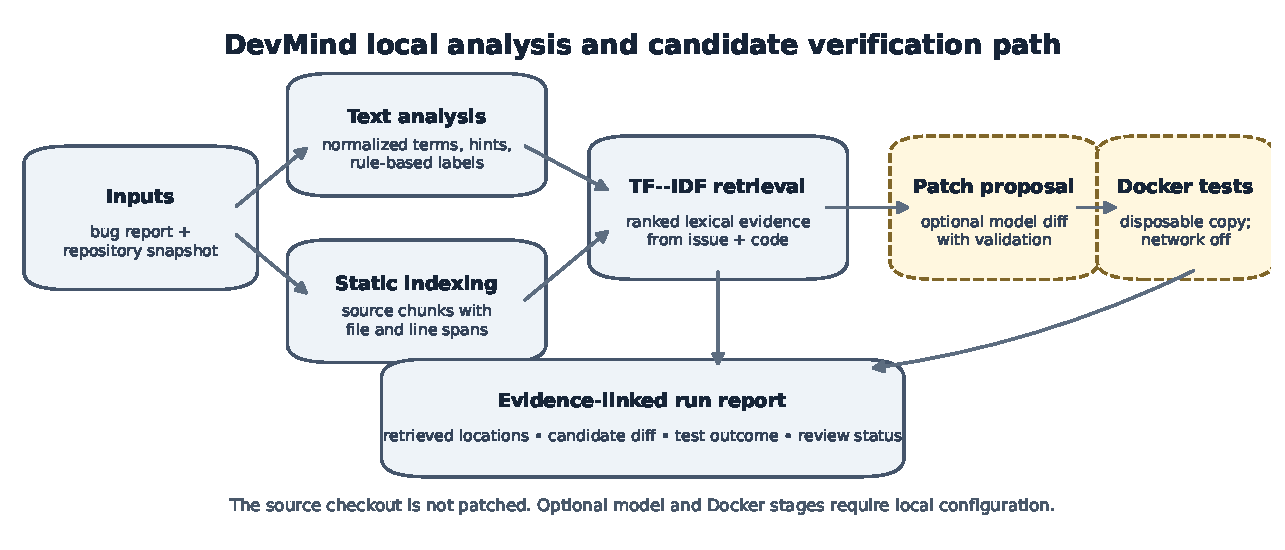
\includegraphics[width=\linewidth]{figures/devmind-architecture.pdf}
\caption{Implemented DevMind analysis path. Optional model generation and sandbox tests require local configuration.}
\label{fig:architecture}
\end{figure}

The architecture keeps static repository analysis available without a model provider. Candidate generation and Docker verification are optional stages, and a generated change remains subject to human review.

\section{Methodology}
\subsection{Issue-text analysis and query conditions}
The Task Analyzer normalizes input text, splits common snake-case and camel-case identifiers, removes configured stop words, ranks terms by frequency, extracts code-like component hints, and assigns an issue category through transparent token rules. It is deterministic; it is not a trained machine-learning model, named-entity recognizer, sentiment model, or topic model. No independently labelled issue corpus has been used to estimate its classification precision, recall, or F1.

A separate \texttt{\detokenize{devmind-query-v1}} experiment preserves the original issue and creates four reproducible conditions: raw text; normalized text; normalized text with extracted keywords and identifiers; and that structured form with observed component/path hints and a non-default rule category when available. No component name or category is guessed. Each record includes the complete transformation trace and generated query. These are study conditions, not evidence that query enrichment improves retrieval.

\subsection{Retrieval methods and metrics}
The application defaults to sparse TF--IDF vectors ranked by cosine similarity. A controlled evaluator separately implements Okapi BM25 with $k_1=1.5$ and $b=0.75$, plus equal-weight reciprocal-rank fusion (RRF) of the TF--IDF and BM25 rankings using a fixed constant of 60. The RRF score is a rank-fusion score, not a similarity. The dense comparison used \texttt{\detokenize{sentence-transformers/all-MiniLM-L6-v2}} at pinned revision \texttt{\detokenize{1110a243fdf4706b3f48f1d95db1a4f5529b4d41}} (384 dimensions) and exact NumPy cosine; a lexical-semantic RRF hybrid was also measured. The model is optional and is not downloaded automatically by the evaluator.

For file-level scoring, each method ranks the same ordered chunks, and duplicate chunks from one file collapse to each file's first occurrence. The evaluator records Precision@1/3/5, Recall@1/3/5, MRR, nDCG@1/3/5, retrieval latency, per-method index-build time, evidence spans, and a whitespace-token estimate of selected source text. The estimate is not an LLM tokenizer count. The dense run additionally records sampled process-tree RSS; a 25 ms sampling interval can miss brief peaks. Pure 	exttt{encode} time is not isolated: index-build timing includes document encoding and vector preparation, while query timing includes query embedding and retrieval.

\section{System Implementation}
\subsection{Static repository indexing}
DevMind discovers supported source files under configured bounds. Python functions and classes are extracted using the Python abstract syntax tree; JavaScript and TypeScript extraction uses lexical structure, including inline scripts in HTML. The indexer recognizes additional languages, but extraction and test-runner support vary. Repository files are treated as untrusted data and are not imported or executed during indexing. Retrieved items preserve file paths, symbols, line spans, and snippets.

\subsection{Investigation and patch proposal}
The deterministic planner creates a bounded checklist from the issue analysis. The investigation stage returns ranked evidence and uncertainty statements; an optional configured provider may generate hypotheses that cite evidence identifiers. A separate optional code-generation path can request a unified diff. Diff validation rejects malformed or unsafe paths, and the candidate is kept outside the selected source checkout. These components form an orchestrated workflow, but the Task Analyzer and planner are rules-based and should not be presented as independent trained agents.

Figure~\ref{fig:repair-workflow} shows the candidate validation path and its bounded retry boundary.
\begin{figure}[t]
\centering
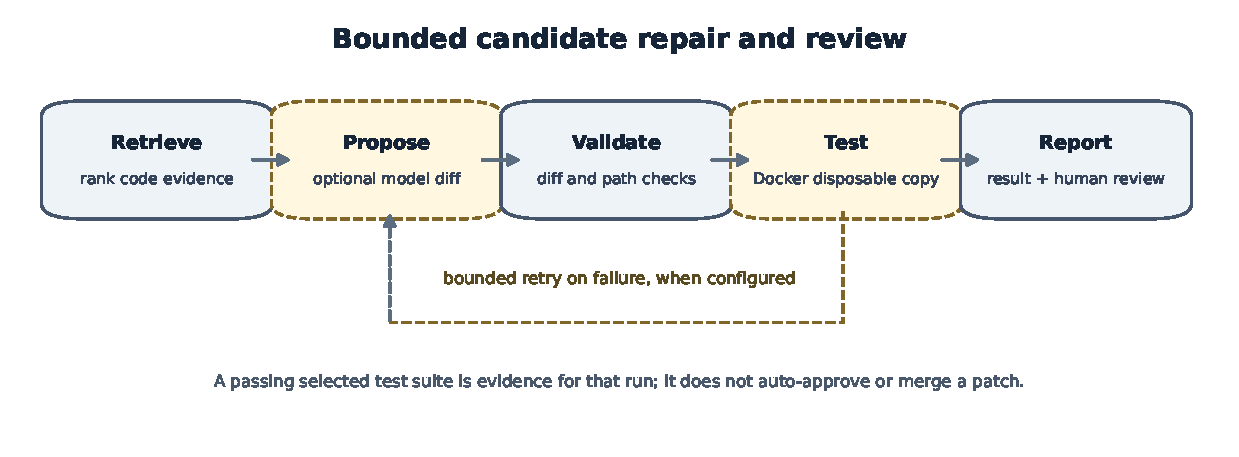
\includegraphics[width=\linewidth]{figures/devmind-repair-workflow.pdf}
\caption{Bounded candidate repair flow. A passing selected test suite remains subject to human review.}
\label{fig:repair-workflow}
\end{figure}

\subsection{Disposable test boundary and reporting}
When Docker and a compatible sandbox image are configured, DevMind copies the repository into a temporary workspace, disables networking, drops Linux capabilities, enables \texttt{\detokenize{no-new-privileges}}, mounts a read-only container root with bounded writable tmpfs, applies CPU, memory, process, and time limits, and tests the candidate only in the disposable copy. The supplied images still run as root. These controls reduce exposure but are not a formal isolation guarantee. A later synthetic Docker smoke exercised the Node image, baseline failure, known candidate pass, and deterministic two-attempt retry; it did not test malicious repositories or verify isolation against an adversary. The images run as root.

The comparison runner first attempts the unmodified test suite once per issue, then runs LLM-only, one-shot RAG, and iterative DevMind. Every valid candidate is tested through the same Docker interface; the iterative method applies that interface on each bounded attempt. Baseline and candidate outcomes remain separate. A missing engine or OS-level launch error produces a blocked result, never a passing test. Raw records capture actual provider calls, prompt character and whitespace-token estimates, sandbox calls, output, and latency. The three conditions have intentionally different evidence and retry behavior; matching snapshots, model settings, task budgets, and independent outcome labels is still required before a fair empirical comparison can be claimed.

A passing result is labelled \texttt{\detokenize{tests_passed_review_required}}; final human review is still necessary. Passing selected tests does not establish that an issue is completely resolved.

\subsection{Repository intake}
The local application accepts a repository folder or public GitHub URL. For a public URL, it resolves the default branch to a full commit SHA, fetches that exact bounded archive, records the archive SHA-256 in the run report, and analyzes extracted files locally without executing downloaded code. A live static-import check on the two presentation repositories reproduced the same commits, archive hashes, and evidence rankings in a second run. Those current revisions already contain the described cart-persistence and single-ball behaviors, so this check validates import and retrieval, not bug repair. Private repository access and hosted service operation are outside scope. A Manifest V3 browser-extension prototype can open the local application and prefill a public GitHub repository URL; it is not a store-published extension.

\section{Dataset and Experimental Setup}
The retrieval experiment used five SWE-bench Lite development instances selected from five distinct repositories. Each repository was pinned to its task base commit and snapshot SHA-256; the exact commit IDs and digests are listed in the reproducibility record and raw-run metadata. The five proxy paths came from fixing-patch changed paths. There is one binary file-level proxy per issue, no reviewer or confidence annotation, and no function-level or independently adjudicated fault-location label. Fixing commits and patches were excluded from evaluator inputs and source snapshots. The environment was Python 3.12.5 on Windows 11 build 26300, Sentence Transformers 5.7.0, Transformers 4.57.6, PyTorch 2.13.0+cpu, and NumPy 2.2.2. CPU inference used ten PyTorch threads; CUDA and FAISS were unavailable. A focused regression command after the evaluator changes, \texttt{\detokenize{.venv\Scripts\python.exe -m pytest tests/test_embeddings.py tests/test_retrieval_experiment.py tests/test_retrieval_evaluation_cli.py --tb=short -rs}}, returned 13 passed in 0.70 second. After subsequent retry and sandbox-output changes, the full suite returned 178 passed and 3 skipped in 5.75 seconds; all skips require Windows symlink-creation permission.

Two saved synthetic-fixture reports record selected tests passing: two tests for a Python calculator candidate and one Node test for a JavaScript cricket-scorer candidate. Those older records do not preserve the Docker image or container command, so they do not independently prove sandbox execution. Both candidates require human review; neither is real issue-localization data or evidence of general repair accuracy. They are excluded from any aggregate repair rate. The provided public QuickCart and Cricket Scorer repositories were not modified, and the demo bug was not confirmed in the selected public source revisions.

The SWE-bench Lite adapter consumes exported JSONL data and explicit task IDs. Two historical exploratory tasks did not yield a usable candidate: the local model timed out on Astropy issue \texttt{\detokenize{astropy__astropy-12907}} and did not return a valid diff for Django issue \texttt{\detokenize{django__django-11179}}. No official harness grading was performed. No benchmark resolution number is available.

The paired retrieval evaluation used identical issue text, four query variants, five base snapshots, top-k=5, and proxy labels for TF--IDF, dense cosine, and lexical-semantic RRF. All 100 dense-run records verified their snapshot hashes. The fixing metadata was not available to the ranking path. The retrieval pilot does not evaluate patch generation or issue resolution, and no significance test is reported.

\section{Results and Evaluation}
Table~\ref{tab:dense} reports the mean over five issues for each method and query condition. Each issue has one proxy file. These values describe agreement with changed-file proxies, not confirmed fault-localization accuracy.


\begin{table}[t]
\caption{Matched dense retrieval comparison, mean across five proxy-labeled issues.}
\label{tab:dense}
\centering
\small
\resizebox{\linewidth}{!}{%
\begin{tabular}{llrrrrr}
\toprule
Query & Method & P@1 & P@5 & R@5 & MRR & nDCG@5 \\
\midrule
Raw & TF--IDF & 0.400 & 0.160 & 0.800 & 0.550 & 0.612 \\
Raw & Dense cosine & 0.400 & 0.080 & 0.400 & 0.400 & 0.400 \\
Raw & Lexical-semantic RRF & 0.400 & 0.120 & 0.600 & 0.440 & 0.477 \\
Normalized & TF--IDF & 0.400 & 0.160 & 0.800 & 0.550 & 0.612 \\
Normalized & Dense cosine & 0.400 & 0.080 & 0.400 & 0.400 & 0.400 \\
Normalized & Lexical-semantic RRF & 0.400 & 0.120 & 0.600 & 0.440 & 0.477 \\
Keywords/IDs & TF--IDF & 0.400 & 0.160 & 0.800 & 0.567 & 0.626 \\
Keywords/IDs & Dense cosine & 0.400 & 0.080 & 0.400 & 0.400 & 0.400 \\
Keywords/IDs & Lexical-semantic RRF & 0.400 & 0.080 & 0.400 & 0.400 & 0.400 \\
Structured & TF--IDF & 0.400 & 0.160 & 0.800 & 0.567 & 0.626 \\
Structured & Dense cosine & 0.400 & 0.080 & 0.400 & 0.400 & 0.400 \\
Structured & Lexical-semantic RRF & 0.400 & 0.080 & 0.400 & 0.400 & 0.400 \\
\bottomrule
\end{tabular}}
\end{table}

Dense cosine matched TF--IDF at P@1 but returned half as many proxy files in the top five on average. It had lower R@5, MRR, and nDCG@5 in all four query conditions. The lexical-semantic hybrid also scored below TF--IDF.

\begin{table}[t]
\caption{Additional project evidence and its limits as of 17 November 2026.}
\label{tab:evidence}
\centering
\small
\begin{tabular}{p{0.20\linewidth}p{0.28\linewidth}p{0.42\linewidth}}
\toprule
Evidence & Recorded outcome & Interpretation and limit \\
\midrule
Focused retrieval regression & 13 passed & Evaluator, embedding adapter and ranking regressions; not the full application suite. \\
Python synthetic repair & 2 selected tests passed in saved report & Docker invocation is not recorded; human review required; not a real issue success. \\
JavaScript synthetic repair & 1 Node test passed in saved report & Docker invocation is not recorded; human review required; not a general repair result. \\
Retrieval pilot & 5 issues; 5 weak proxy labels & Matched dense and lexical rankings; no reviewed localization or repair outcomes. \\
Repair comparison & No matched model-backed runs & No resolution accuracy or workflow comparison. \\
SWE-bench Lite smoke & Two exploratory attempts; no usable patch; harness not run & No benchmark tasks graded and no score. \\
Task Analyzer quality & No independently labelled corpus & Classification precision, recall, and F1 are unknown. \\
\bottomrule
\end{tabular}
\end{table}

The raw and derived records support the five-case retrieval comparison. The observed result favors TF--IDF on top-five agreement and ranking metrics, while dense retrieval required substantially more CPU time and memory. Historical fixture tests show only that two candidate changes passed selected tests in specific disposable environments; they do not establish general repair accuracy.

\section{Discussion and Limitations}
The current evidence supports an implemented prototype with deterministic text analysis, traceable lexical retrieval, optional model proposals, bounded repair orchestration, and Docker-only candidate testing when the engine is available. The app's default remains TF--IDF. The dense route was exercised in a pinned five-repository CPU pilot. On this sample it did not improve proxy localization and incurred much higher indexing cost. The literature already covers query reformulation, semantic/hybrid localization, evidence-gated repair, and localization-to-repair effects. DevMind does not claim novelty for those ideas.

The empirical record remains small and the localization annotations are weak. One changed-file proxy per issue may not identify the actual fault location; no labels are independently reviewed or function-level, so incomplete ground truth can penalize a valid alternate location. Memory is sampled RSS and may miss brief peaks. Pure model-only encode time was not isolated. The run measured retrieval/indexing, not generated patches or repair success. Results should not be generalized beyond these five repositories, one general-purpose embedding model, CPU hardware, and the recorded query conditions.

The sandbox reduces risk using a disposable copy, network isolation, capability dropping, \texttt{\detokenize{no-new-privileges}}, a read-only root, resource limits, and timeouts. The provided images still run as root. A synthetic live Docker smoke verified startup, a known candidate test, bounded output, and the deterministic retry path; it is not a formal isolation assessment and does not verify model-generated repair. The project also lacks \texttt{\detokenize{.git}} metadata, so a branch or source commit cannot be recorded. The retrieval study itself does not measure patch testing or issue resolution.

\section{Conclusion and Future Work}
DevMind combines rule-based bug-report analysis, repository-aware evidence retrieval, optional model-generated candidate patches, and bounded disposable testing in a local tool. In the five-case retrieval pilot, dense cosine did not improve agreement with the available changed-file proxies over TF--IDF and cost substantially more to index. The small, weakly labeled sample does not establish general superiority of lexical retrieval, and retrieval metrics do not establish repair success. No official SWE-bench grade exists. The project remains an educational prototype with an initial reproducible localization evaluation, not a proven autonomous repair system.

The next research step is to improve annotation coverage: independently review multiple relevant files and function-level locations, preserve uncertainty, and distinguish the true fault location from files changed by a fix. Then expand the pinned repository sample and repeat the same paired retrieval protocol. Repair comparison requires a fixed model and configuration, equal task/test conditions, a working Docker engine, and independent resolution adjudication.

\appendix
\section{Recorded Reproduction Details}
Exact commands, raw JSONL records, repository commits and snapshot hashes, model identity, and integrity checks are in the accompanying reproducibility record and manifests. The full project regression suite was run on 17 November 2026 and returned 179 passed and 3 skipped in 5.73 seconds; the skips require Windows symlink-creation permission.

\section*{Acknowledgements}
The authors thank [faculty guide name] and the Department of Computer Science and Engineering at [college/university] for their guidance. % Confirm wording before submission.

\begin{thebibliography}{99}
\bibitem{Lewis2020}
P. Lewis, E. Perez, A. Piktus, F. Petroni, V. Karpukhin, N. Goyal, H. K\"uttler, M. Lewis, W. Yih, T. Rockt\"aschel, S. Riedel, and D. Kiela, ``Retrieval-Augmented Generation for Knowledge-Intensive NLP Tasks,'' in \emph{Advances in Neural Information Processing Systems}, vol. 33, 2020.

\bibitem{Jimenez2024}
C. E. Jimenez, J. Yang, A. Wettig, S. Yao, K. Pei, O. Press, and K. Narasimhan, ``SWE-bench: Can Language Models Resolve Real-World GitHub Issues?'' in \emph{International Conference on Learning Representations}, 2024.

\bibitem{Yang2024}
J. Yang, C. E. Jimenez, A. Wettig, K. Lieret, S. Yao, K. Narasimhan, and O. Press, ``SWE-agent: Agent-Computer Interfaces Enable Automated Software Engineering,'' in \emph{Advances in Neural Information Processing Systems}, vol. 37, 2024.

\bibitem{Zhang2024}
Y. Zhang, H. Ruan, Z. Fan, and A. Roychoudhury, ``AutoCodeRover: Autonomous Program Improvement,'' in \emph{Proceedings of the 33rd ACM SIGSOFT International Symposium on Software Testing and Analysis}, pp. 1592--1604, 2024, doi: 10.1145/3650212.3680384.

\bibitem{RepairAgent2025}
I. Bouzenia, P. Devanbu, and M. Pradel, ``RepairAgent: An Autonomous, LLM-Based Agent for Program Repair,'' in \emph{Proceedings of the IEEE/ACM 47th International Conference on Software Engineering}, pp. 2188--2200, 2025, doi: 10.1109/ICSE55347.2025.00157.

\bibitem{RepoAI2026}
N. Chondamrongkul, M. P. P. Kyaw, S. M. Ko, P. P. Paing, M. K. T. Swe, and T. Hongthong, ``RepoAI: Automated code refactoring through multi-agent LLM orchestration and retrieval-augmented generation,'' \emph{Science of Computer Programming}, vol. 253, article 103477, Aug. 2026, doi: 10.1016/j.scico.2026.103477.

\bibitem{Andrade2026}
R. Andrade, C. Teixeira, N. Laranjeiro, and M. Vieira, ``An Empirical Study on the Classification of Bug Reports with Machine Learning,'' \emph{IEEE Open Journal of the Computer Society}, vol. 7, pp. 1213--1224, 2026, doi: 10.1109/OJCS.2026.3692087. First published 11 May 2026; author preprint arXiv:2503.00660.

\bibitem{Long2025}
G. Long, J. Gong, H. Fang, and T. Chen, ``Learning Software Bug Reports: A Systematic Literature Review,'' \emph{ACM Transactions on Software Engineering and Methodology}, 2025, doi: 10.1145/3750040.

\bibitem{Agentless2025}
C. S. Xia, Y. Deng, S. Dunn, and L. Zhang, ``Agentless: Demystifying LLM-Based Software Engineering Agents,'' in \emph{Proceedings of the ACM International Conference on the Foundations of Software Engineering}, 2025. Preprint: arXiv:2407.01489.

\bibitem{BRaIn2025}
A. M. Samir and M. M. Rahman, ``Improved IR-based Bug Localization with Intelligent Relevance Feedback,'' arXiv preprint arXiv:2501.10542, 2025.

\bibitem{Reformulate2026}
G. Caumartin and G. Melo, ``Reformulate, Retrieve, Localize: Agents for Repository-Level Bug Localization,'' in \emph{Proceedings of the 2026 IEEE/ACM International Workshop on Bots and Agents in Software Engineering (BotSE)}, 2026. Preprint: arXiv:2512.07022. URL: \url{https://conf.researchr.org/details/icse-2026/botse-2026-papers/5/Reformulate-Retrieve-Localize-Agents-for-Repository-Level-Bug-Localization}.

\bibitem{IQLoc2026}
A. M. Samir and M. M. Rahman, ``Improving IR-based Bug Localization with Semantics-Driven Query Reduction,'' \emph{Journal of Systems and Software}, vol. 237, article 112860, 2026, doi: 10.1016/j.jss.2026.112860.

\bibitem{SpIDER2026}
S. S. Chaudhari, R. T. Jacob, J. Cao, M. S. Rashid, M. Goswami, and C. Bock, ``SpIDER: Spatially Informed Dense Embedding Retrieval for Software Issue Localization,'' in \emph{Proceedings of the 2026 Conference on Empirical Methods in Natural Language Processing}, pp. 44096--44131, 2026. URL: \url{https://aclanthology.org/2026.emnlp-main.1938/}.

\bibitem{EviACT2026}
Q. Meng, X. Zhang, Z. Ren, and J. Visser, ``EviACT: An Evidence-to-Action Framework for Agentic Program Repair,'' arXiv preprint arXiv:2605.27238, 2026.

\bibitem{Loc2Repair2026}
M. N. Al Awad and S. Ivanov, ``Loc2Repair: A Framework for Evaluating the Impact of File-Level Issue Localization in Repo-Level LLM Repair,'' arXiv preprint arXiv:2606.30963, 2026.
\end{thebibliography}

\end{document}
